\documentclass[t]{sdqbeamer}
%\documentclass[c]{sdqbeamer}

\usepackage{listings}
\usepackage{graphicx}
\usepackage{tabularx}
\usepackage{tikzsymbols}
\usepackage[lined,linesnumbered,ruled,noend]{algorithm2e}

\hypersetup{
	colorlinks=true,
	urlcolor=kit-orange
}

% set sdqbeamer options
\titleimage{blender-render}
\groupname{Algorithm Engineering}
\grouplogo{ae}
\selectlanguage{english}

% define title etc.pp.
\title[SAT Solving]{Practical SAT Solving}
\subtitle{Exercise 1}
\author{\underline{Markus Iser}, Dominik Schreiber, Tom\'a\v{s} Balyo}
\date{April 23, 2024}

% Existing KIT colors: kit-green, kit-blue, kit-red, kit-gray, kit-orange, kit-lightgreen, kit-brown, kit-purple, kit-cyan
% configure appearance
\setbeamercolor{block title}{bg=kit-blue}
\setbeamercolor{block body}{bg=kit-blue!10}
\setbeamercolor{block title example}{bg=kit-orange}
\setbeamercolor{block body example}{bg=kit-orange!10}
\setbeamertemplate{itemize item}{\color{kit-gray}\textbullet}
\setbeamertemplate{itemize subitem}{\color{kit-gray}\textbullet}
\setbeamercolor{item projected}{bg=kit-gray, fg=kit-gray}
\renewcommand{\insertnavigation}[1]{} % remove navigation bar

% define commands
\definecolor{myblue}{HTML}{0D3B66}
\definecolor{myred}{HTML}{6E0E0A}
\definecolor{mypink}{HTML}{F7B2B7}

\newcommand{\vars}[1]{\textsf{vars} (#1)}
\newcommand{\lits}[1]{\textsf{lits} (#1)}
\newcommand{\clss}[1]{\textsf{clss} (#1)}

\newcommand{\highl}[1]{\textcolor{myblue}{#1}}
\newcommand{\highlo}[1]{\textcolor{myred}{#1}}
\newcommand{\highlow}[1]{\textcolor{mypink}{#1}}

% Extra column types for tabularx
\newcolumntype{C}{>{\centering\arraybackslash}X}
\newcolumntype{L}{>{\raggedright\arraybackslash}X}
\newcolumntype{R}{>{\raggedleft\arraybackslash}X}

\newcommand{\setcolsep}[1]{\setlength{\tabcolsep}{#1}}
\newcommand{\setrowsep}[1]{\renewcommand{\arraystretch}{#1}}

% Definitions for the Tseitin transformation
\newcommand{\true}{\ensuremath{\mathit{True}}}
\newcommand{\false}{\ensuremath{\mathit{False}}}
\newcommand{\allvars}{\ensuremath{\mathcal{V}}}
\newcommand{\tseitin}[1]{\ensuremath{\mathcal{T}(#1)}}
\newcommand{\tseitinRec}[2]{\ensuremath{\mathcal{T}^{#2}(#1)}}
\newcommand{\tseitinSym}[1]{\ensuremath{\mathcal{T}_\mathsf{lit}(#1)}}
\newcommand{\tseitinDef}[2]{\ensuremath{\mathcal{T}_\mathsf{def}^{#2}(#1)}}
\newcommand{\hcancel}[2][black]{\setbox0=\hbox{$#2$}\rlap{\raisebox{.45\ht0}{\textcolor{#1}{\rule{\wd0}{1pt}}}}#2} 
\newcommand{\sateq}{\mathrel{\overset{\makebox[0pt]{\mbox{\normalfont\tiny\sffamily SAT}}}{=}}}

\newcommand{\enc}{\ensuremath{\mathcal{E}}} % encoding

% exercise commands
\newcommand{\exhead}[3]{
\hrule~\\[1ex]\noindent
{\bf Practical SAT Solving} (ST 2024) \hfill \fbox{Assignment #1} \\[1ex]
Markus Iser, Dominik Schreiber, Tom\'a\v{s} Balyo\\[1ex]
Algorithm Engineering (KIT) \hfill #2 -- #3\\
\hrule
\thispagestyle{empty}
}
\setlength{\itemsep}{1em}

\begin{document}

\begin{frame}
	\thispagestyle{empty}
	\titlepage
\end{frame}

\begin{frame}{Pigeon Hole Principle}
	The pigeonhole principle asserts that there is no injective mapping from $m$ pigeons to $n$ holes as long as $m > n$.
	\begin{center}
		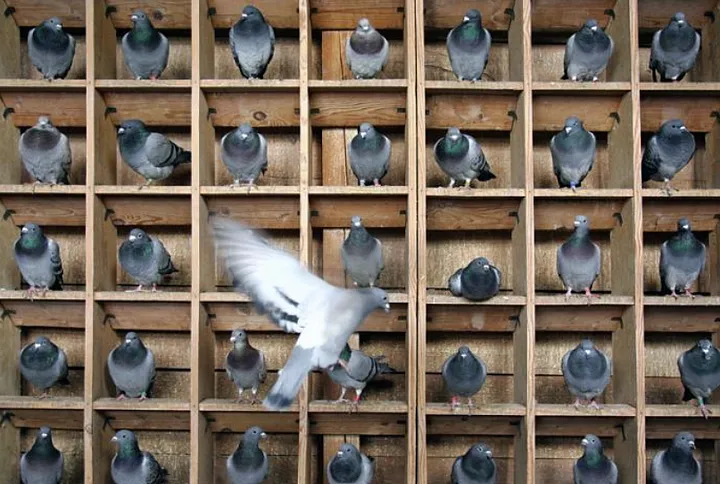
\includegraphics[height=0.6\textheight]{figures/e01/phole.png}~\\
		Image by \url{https://jineralknowledge.com/}
	\end{center}
\end{frame}

\begin{frame}{Assignment 2}
	The next assignment is for four weeks, so you can get twice as many points as usual.
	\begin{block}{Competitions: Tetris Puzzle Encoding and Local Search Solver}
		You can team up with a partner in the competitions. This has some advantages.~\\[1ex]
		\begin{itemize}\setlength{\itemsep}{1ex}
			\item You can discuss the problem with someone else.
			\item You can split the work.
			\item You can learn from each other.
			\item You double your chances of winning the competition.
			\item You double your chances of getting a bonus.
		\end{itemize}
	\end{block}
\end{frame}

\begin{frame}{SLUR Formulas \href{https://doi.org/10.1007/978-3-642-27660-6_15}{(Čepek et al., 2012)}}
	\setlength\columnsep{1ex}
	\begin{columns}
		\begin{column}{.3\linewidth}
			A CNF formula is SLUR if the SLUR algorithm \highl{never gives up} on it \highl{regardless of the non-deterministic choices} in Lines~2 and~8.\\[1ex]

			
		\end{column}
		\begin{column}{.6\linewidth}
			\vspace*{-3ex}
			\renewcommand{\thealgocf}{} % remove algo. numbering

			\LinesNotNumbered
			\begin{algorithm}[H]
				\DontPrintSemicolon
				\SetKwFunction{SLURSAT}{SLURSAT}
				\SetKwFunction{UnitResolution}{UnitResolution}
				\SetKwFunction{UNSAT}{\highlo{UNSAT}}
				$F \leftarrow$ \UnitResolution{$F$} \;
				\lIf {$\bot \in F$} {
					\Return \UNSAT
				}
				\lElse {
					\Return \SLURSAT{$F$}
				}
				\caption{Single-lookahead Unit Resolution (SLUR)}
			\end{algorithm}

			\LinesNumbered
			\begin{algorithm}[H]
				\DontPrintSemicolon
				\SetAlgorithmName{Function}{function}{List of Functions}

				\SetKwFunction{SLUR}{SLUR}
				\SetKwFunction{UnitResolution}{UnitResolution}
				\SetKwFunction{SelectVariable}{SelectVariable}
				\SetKwFunction{GIVEUP}{\highlo{GIVE-UP}}
				\SetKwFunction{SAT}{\highlo{SAT}}
				
				\lIf {all variables appear in a unit clause} {
					\Return \SAT
				}

				$v \leftarrow$ \SelectVariable{$F$} \tcp*{non-det. choice}
				$F_1 \leftarrow$ \UnitResolution{$F \land (v)$} \;
				$F_2 \leftarrow$ \UnitResolution{$F \land (\overline{v})$} \;

				\lIf {$\bot \in F_1$ \textbf{and} $\bot \in F_2$} {
					\Return \GIVEUP
				}
				\lIf {$\bot \in F_1$ \textbf{and} $\bot \notin F_2$} {
					\Return \SLUR{$F_2$}
				}
				\lIf {$\bot \notin F_1$ \textbf{and} $\bot \in F_2$} {
					\Return \SLUR{$F_1$}
				}
				\Return \SLUR{$F_1$} \textbf{non-det. or} \SLUR{$F_2$} \tcp*{non-det. choice}

				\caption{SLURSAT}
			\end{algorithm}
		\end{column}
	\end{columns}
\end{frame}

\begin{frame}{Properties of SLUR Formulas}
	\begin{itemize}\setlength{\itemsep}{1em}
		\item Solvable in \highl{polynomial time} (using the SLUR algorithm)
		\item SLUR is an \highl{umbrella class for polynomially solvable classes}
		\begin{itemize}
			\item All \highl{Horn and Hidden Horn} formulas are SLUR formulas
			\item Also true for Extended Horn, Balanced, and Propagation Complete formulas
		\end{itemize}
		\item It is \highlo{co-NP-complete} to recognize whether a given CNF is a SLUR formula or not
	\end{itemize}
\end{frame}

% \begin{frame}{Integer Multiplication / Factorization}
% 	\begin{center}
% 		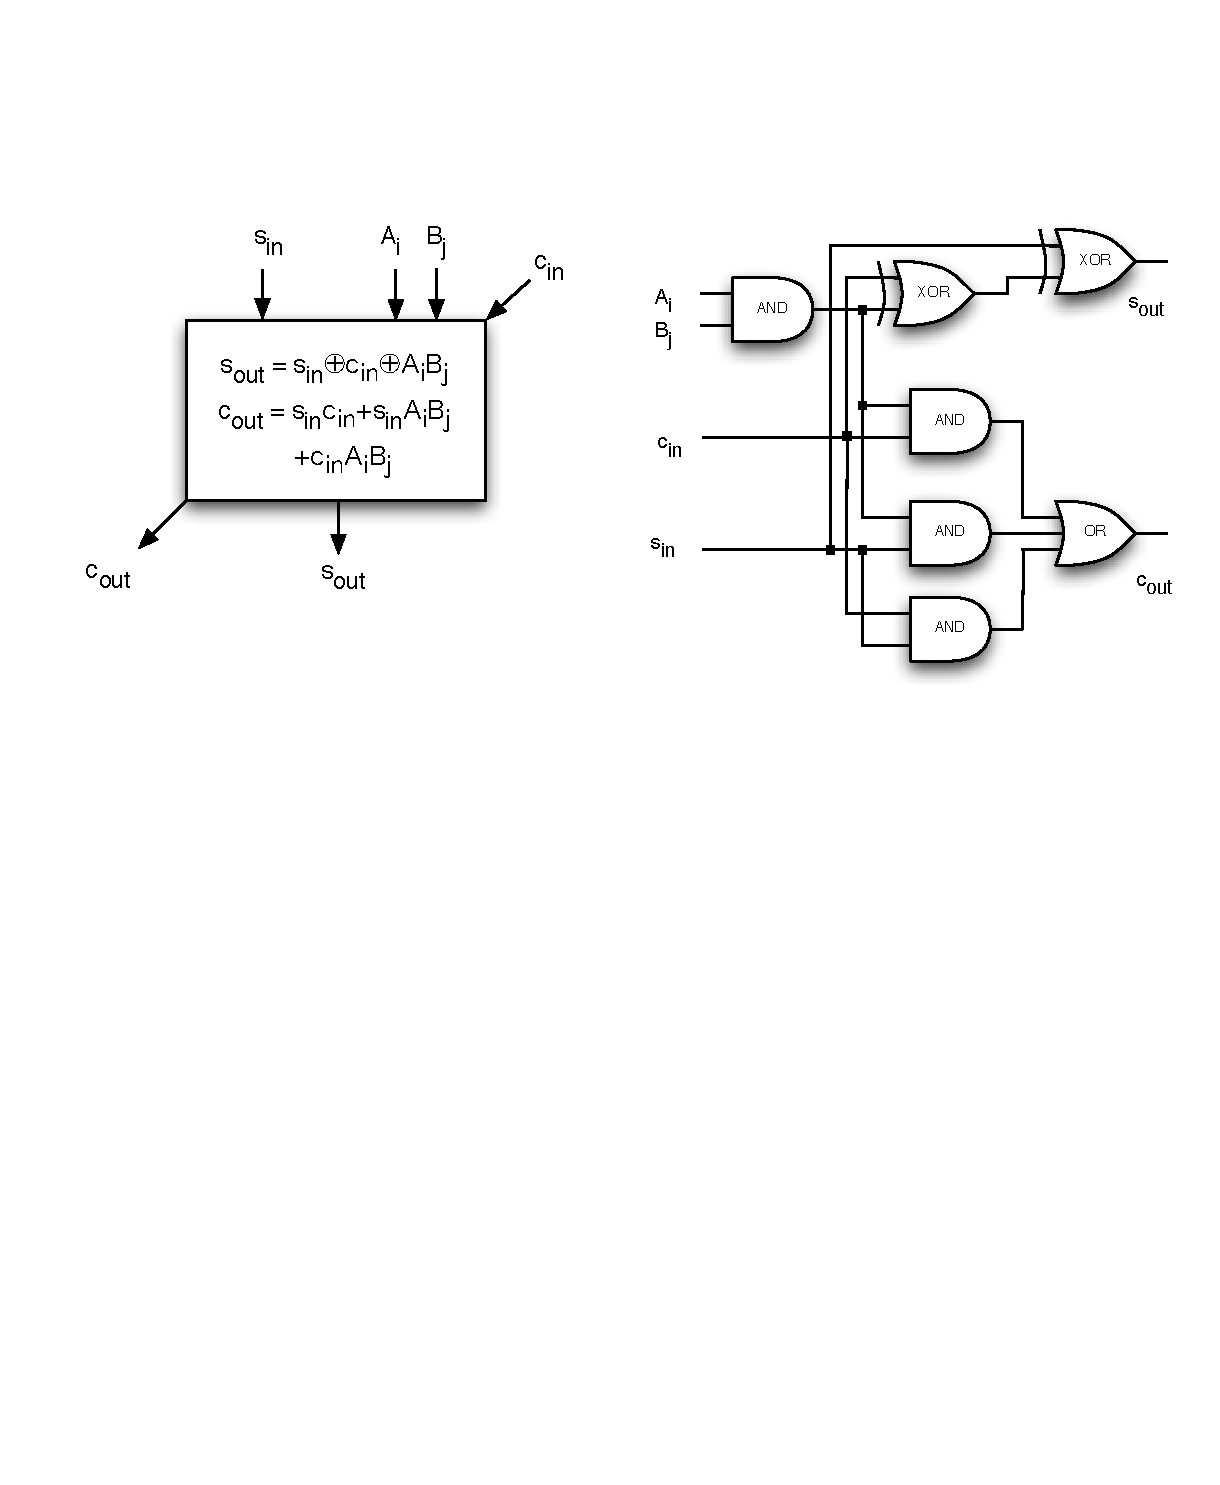
\includegraphics[height=0.4\textheight]{figures/l02/multiplier-1.pdf} \\
% 		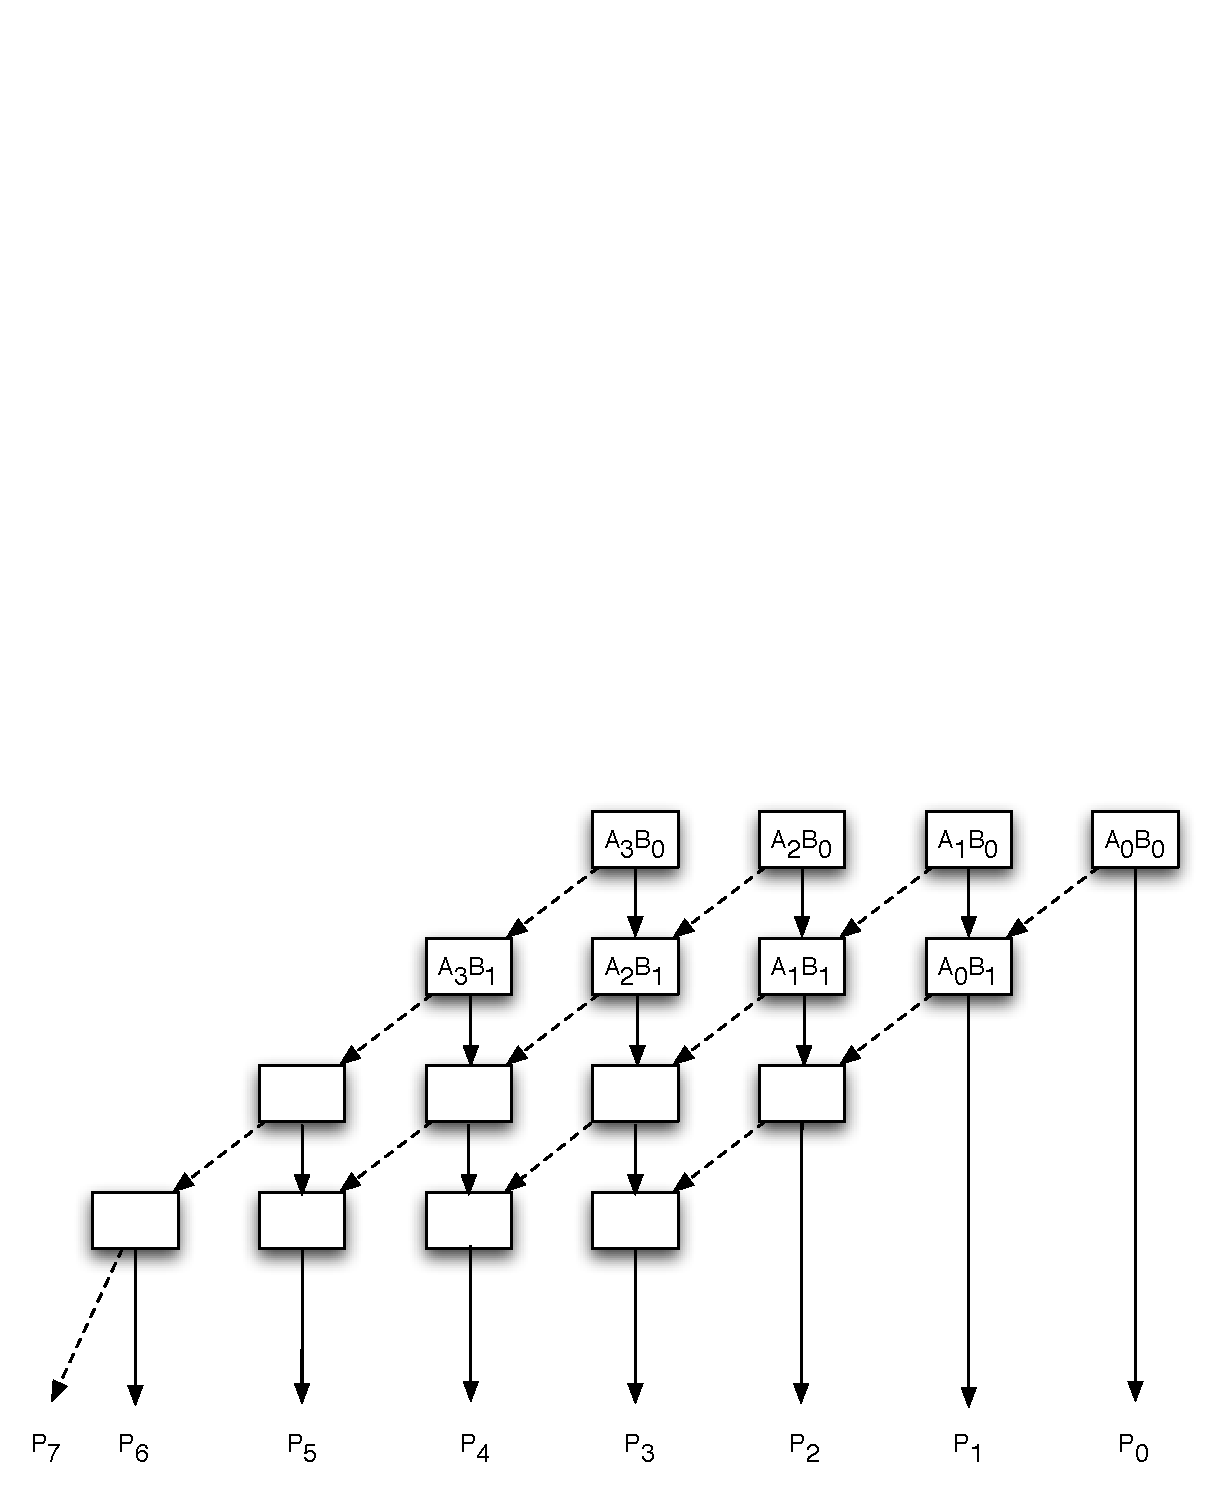
\includegraphics[height=0.4\textheight]{figures/l02/multiplier-2.pdf}
% 	\end{center}
% \end{frame}

\end{document}
